\section{ChimeraX Map Subtraction protocol}
\label{app:chimeraMapSubtraction}%a013

\chimera-based protocol designed to subtract two maps. These two maps can be two density maps experimentally obtained or derived from different computations, including the generation of a density map from an atomic structure. In the context of the \scipion modeling workflow this protocol helps to find out unmodeled densities in a map as a whole or in a specific part of it. In addition, wrong modeled regions can be also identified with this protocol since the atomic structure could doesn't fit to the density map.  
   
 \begin{itemize}
  \item Requirements to run this protocol and visualize results:
    \begin{itemize}
        \item \scipion plugin: \ttt{scipion-em}
        \item \scipion plugin: \ttt{scipion-em-chimera}
    \end{itemize}
  \item \scipion menu:
  \ttt{Model building -> Tools-Calculators} (\ffigure{fig:app_protocol_map_subtract_1} (A))
  
    \begin{figure}[H]
    \centering 
    \captionsetup{width=.9\linewidth} 
    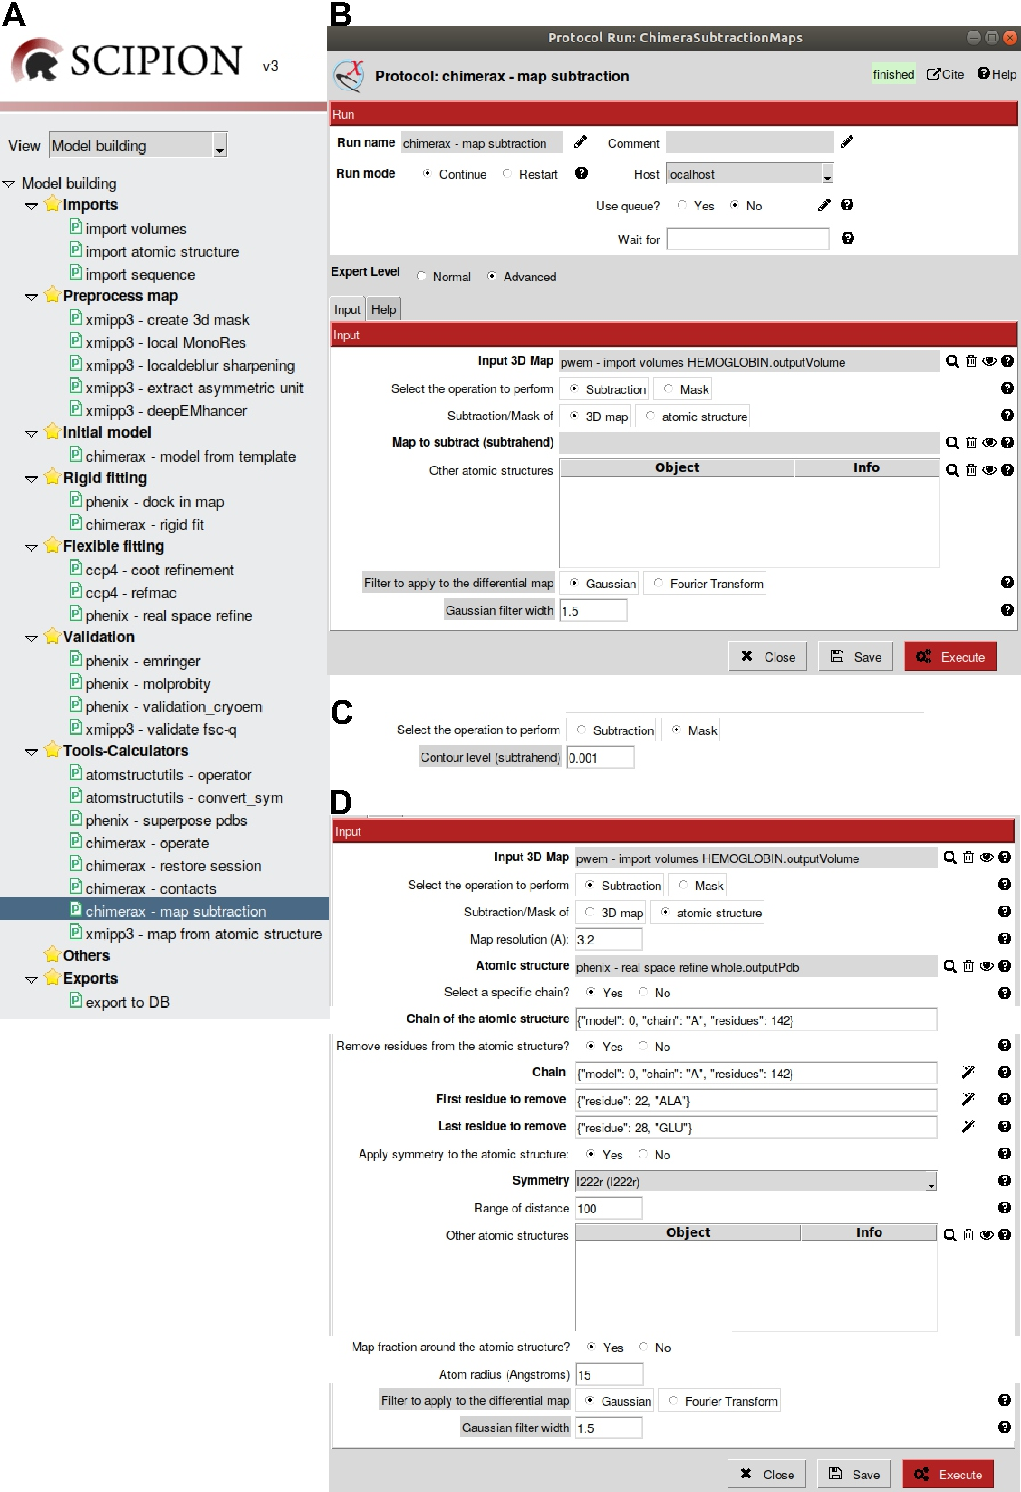
\includegraphics[width=0.85\textwidth]{Images_appendix/Fig309.pdf}
    \caption{Protocol \scommand{chimerax - map subtraction}. A: Protocol location in \scipion menu. B: Protocol form to subtract two maps. C: Param option \ttt{Mask}. D: Protocol form to subtract an atomic structure from a map. All possible params are shown. }
    \label{fig:app_protocol_map_subtract_1}
   \end{figure}
  
  \item Protocol form parameters (\ffigure{fig:app_protocol_map_subtract_1} (B,C,D)):\\ \ttt{Input} section:  

  \begin{itemize}
   \item \ttt{Input 3D Map}: Include here any map previously downloaded or generated in \scipion that you would like to use as minuend of the subtraction operation.
   \item \ttt{Select the operation to perform}: Two possibilities are allowed:
    \begin{itemize}
    \item \ttt{Subtraction}: Between minuend and subtrahend maps, and you'll obtain the difference.
    \item \ttt{Mask}: The voxel region of the subtrahend greater than a certain level will be masked (\ffigure{fig:app_protocol_map_subtract_1} (C)). The default level is \ttt{0.001} although can be modified with the \ttt{Advanced} param \ttt{Contour level (subtrahend)}. If no level is supplied, \chimerax will compute that level value.
    \end{itemize}
   \item \ttt{Subtraction/Mask of}: Select the subtrahend of the subtraction operation. Two possibilities are allowed:
    \begin{itemize}
   \item \ttt{3D map}: Any map previously downloaded or generated in \scipion. WARNING: The sampling rate of this map should be identical to the subtrahend's.
   \item \ttt{atomic structure}: Previously downloaded or generated in \scipion. By selecting this option many new params will interrogate about the structure-derived map that you would like to generate (\ffigure{fig:app_protocol_map_subtract_1} (D)).
            \begin{itemize}
            \item \ttt{Map resolution (\AA)}: This is a tricky param and a uniform rule cannot be followed since, although its value is related with the minuend map resolution obtained by computing the \ttt{FSC} in the reconstruction process, local variations of this resolution seem to be involved. As a general rule, start with a resolution value half of the one obtained by the \ttt{FSC} and check your results. Then test other resolution values closer to the one computed by the \ttt{FSC} and compare the results with the previous one. At the end select the resolution that maximizes the difference between the minuend and the subtrahend.
            \item \ttt{Atomic structure}: Select the atomic structure in the \scipion workflow.
            \item \ttt{Select a specific chain?}: In case you are interested in generate the sustrahend \ttt{3D map} from the input atomic structure as a whole, answer \ttt{No} to this question. However, answer \ttt{Yes} if you want to derive that map from a specific chain of the atomic structure. If this is the case, a new param (\ttt{Chain of the atomic structure}) will interrogate you about the specific chain that you can select with the help of the wizard on the right.
            \item \ttt{Remove residues from the atomic structure?}: Select \ttt{Yes} to answer this question in case you'd like to count on a control of density levels to identify the differential density. The aim of this control is identify the density of the removed residues in the differential map. However, be cautious about discarding other densities that could appear in lower resolution areas and have density levels slightly different that the control one. After running the program the \chimera graphics window will open and the atomic structure won't show the removed residues. To make easier the localization of this area, ten residues both upstream and downstream of the removed aminoacids will be highlighted.\\
            Additional params to interrogate about the residues to be removed are \ttt{Chain}, \ttt{First residue to remove} and \ttt{Last residue to remove}. A wizard on the right helps to select this three elements. WARNING: In case you have already selected a specific chain of the structure to generate the \ttt{3D Map}, this chain will appear by default in the param \ttt{Chain} since the selection of a different chain wouldn't make sense.
            \item \ttt{Apply symmetry to the atomic structure}: In case your input atomic structure to derive the subtrahend \ttt{3D map} corresponds to the asymmetric unit and you'd like to have the whole atomic structure or at least several adjacent asymmetric units together with the input one, select the option \ttt{Yes}. Otherwise, the subtrahend derived map will only correspond to the asymmetric unit. All \chimera symmetries will be available (\url{https://www.cgl.ucsf.edu/chimerax/docs/user/commands/sym.html}). In case you select symmetries cyclic or dihedral, an additional param will interrogate you about the \ttt{Symmetry Order}. Pay attention to the param \ttt{Range of distance}, set to \ttt{100} by default. This is the distance (in \AA) from the center of the input asymmetric unit to the center of additional allowed asymmetric units, in order to select only the closer ones. You should probably modify the default value to regenerate big maps by applying symmetry.
            \item \ttt{Map fraction around the atomic structure?}: Select the option \ttt{Yes} if you want to limit the input minuend \ttt{3D Map} to a certain area around the atomic structure. This is the option recommended if you have a big starting map and you'd like to substract a much smaller subtrahend structure-derived map since the visualization of results will be much easier. An additional param, \ttt{Atom radius (\AA)} asks you about the distance around the input structure used to crop the input \ttt{3D Map}. \ttt{15} is the default value.
            \end{itemize}
    \item \ttt{Other atomic structures}: Additional atomic structures previously downloaded or obtained in \scipion can be included here to help you identify particular areas of the map or structure. Then, those structures are only informative and won't be used to generate the subtrahend map.
    \item \ttt{Filter to apply to the differential map}: Since the differential map results usually quite blurry, you can clean it somehow by applying a filter in order to maximize visualization of the differences between the minuend and the subtrahend maps. This 
    \end{itemize}
   \end{itemize}
   
  
  \item Protocol execution:
  
  Adding specific volume label is recommended in \ttt{Run name} section, at the form top. To add the label, open the protocol form, press the pencil symbol at the right side of \ttt{Run name} box, complete the label in the new opened window, press OK, and finally, close the protocol. This label will be shown in the output summary content (see below). If you want to run again this protocol, do not forget to set to \ttt{Restart} the \ttt{Run mode}.\\
  Press the \ttt{Execute} red button at the form bottom.
  
  \item Visualization of protocol results:
  
  After executing the protocol, press \ttt{Analyze Results} and $ShowJ$, the default \scipion viewer, will allow you to visualize the \ttt{slices} window of the map  (\ffigure{fig:app_protocol_assign_orig_and_sampling_2}). The $ShowJ$ window menu (\ttt{File -> Open with ChimeraX}) allows to open the selected map in $ChimeraX$ graphics window.
   
   \begin{itemize}
  \item \ttt{slices}: $ShowJ$
   
\url{https://github.com/I2PC/scipion/wiki/ShowJ}


   \begin{figure}[H]
   \centering 
    \captionsetup{width=.7\linewidth} 
    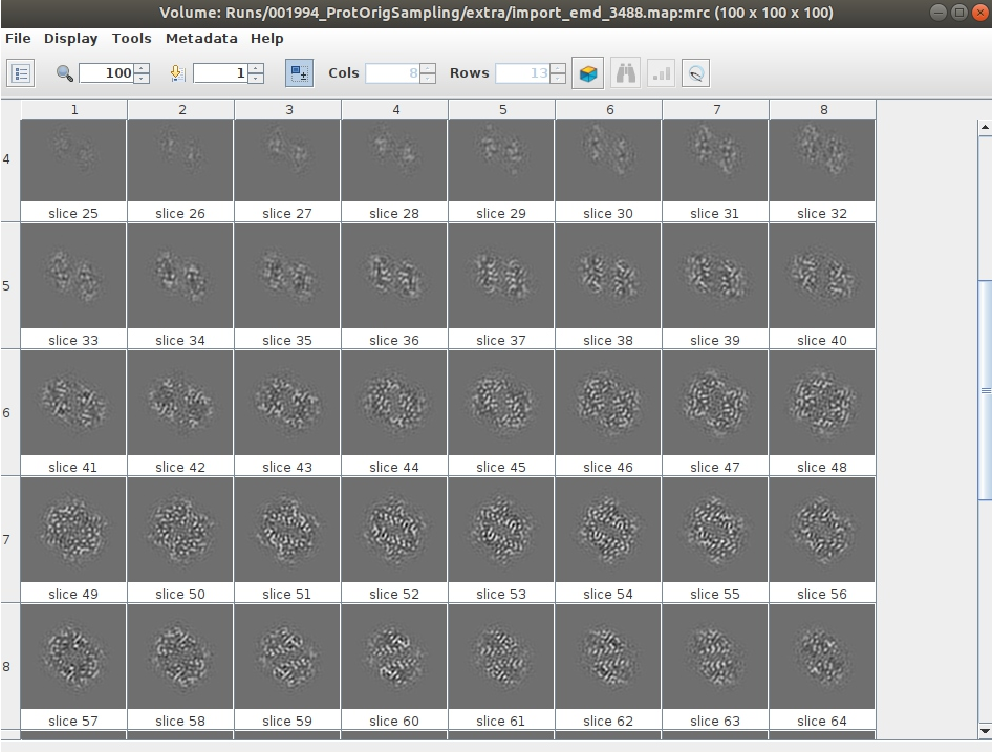
\includegraphics[width=0.75\textwidth]{Images_appendix/Fig302.pdf}
    \caption{Protocol \scommand{assign Orig \& Sampling}. Gallery model of $ShowJ$ to visualize the map slices.}
    \label{fig:app_protocol_assign_orig_and_sampling_2}
   \end{figure}
   
   \end{itemize}
   
   \item Summary content:
    
    \begin{itemize}
     \item Protocol output (below \scipion framework):\\ \ttt{pwem - assign Orig \& Sampling -> ouputVolume};\\ \ttt{Volume (x, y, and z dimensions, NEW sampling rate)}.
     \item \ttt{SUMMARY} box:\\\ttt{New Sampling}: New assigned value of sampling rate.\\\ttt{New Origin}: Coordinates \ttt{x, y, z} of the new assigned origin of coordinates.
    \end{itemize}
  
  \end{itemize}

